\section{Théorie de Morse}

\subsection{Définitions et lemme de Morse}

\subsubsection{Définitions}
\begin{defi}
    Soit $M$ une variété et soit $f:M\to\R$ une application différentiable.
    Un point $x\in M$ tel que la différentielle $\dd f_x:T_xS\to T_{f(x)}\R$ 
    est nulle est appelé point critique. Une valeur critique de $f$ est 
    l'image par $f$ d'un point critique.
\end{defi}

Si $M$ est une surface, en regardant dans une carte $\varphi$ telle que $\varphi(s,t)=x$, 
cela revient à écrire 
\[
    \frac{\partial(f\circ\varphi)}{\partial s}(s,t)=
    \frac{\partial(f\circ\varphi)}{\partial t}(s,t)=0
\]

\begin{defi}
    Soit $M$ une variété.
    Soit $f:M\to \R$ une application lisse, $x$ un point critique de $f$ et $\varphi:U\to V$ 
    une carte de $M$, avec $x\in U$. 
    On définit alors la hessienne de $f$ par rapport à $\varphi$, notée $H_\varphi(f)$, comme 
    étant la hessienne de l'application $f\circ\varphi^{-1}$. 
\end{defi}

\begin{remark}
    En reprenant les éléments de la définition précédente et en prenant $\psi:U'\to V'$ une 
    autre carte avec $x\in U'$, on peut montrer que 
    \[
        H_\varphi(f)={}^tJH_\psi(f)J
    \]
    où $J$ désigne la jacobienne de $\psi\circ\varphi^{-1}$ en $\varphi(x)$.
\end{remark}

\begin{defi}
    Soit $M$ une variété, $f:M\to \R$ une application lisse.
    Soit $x\in M$ un point critique de $f$. 
    On dit que $x$ est un point critique non dégénéré si la forme quadratique associée 
    à la hessienne en $x$ par rapport à n'importe quelle carte dont le domaine contient 
    $x$ est non dégénérée. 
    Son indice sera, de la même manière, l'indice de la forme quadratique associée à une
    hessienne choisie comme précédemment.
\end{defi}

\begin{remark}
    En vertu de la remarque précédente, notre définition est bonne puisque le caractère
    non dégénéré d'un point critique  ne dépend pas de la carte dans laquelle on regarde notre
    fonction.
\end{remark}

\begin{defi}
    Une fonction de Morse est une application lisse $f:M\to \R$, où $M$ est une variété, 
    dont tous les points critiques sont non dégénérés.
\end{defi}

\subsubsection{Lemme de Morse}
\begin{lem}[de Morse à $n$ variables]
    Soit $f:U\to\R$ une fonction lisse avec $U\subset\R^n$ un ouvert contenant $0$. 
    Si $0$ est un point critique non dégénéré de $f$ d'indice $\lambda$, alors il existe un 
    difféomorphisme lisse $\varphi:V\to W$ entre deux voisinages ouverts de l'origine 
    tel que $\varphi(0)=0$ et 
    \[
        f\circ\varphi(x)=f(0)+x_1^2+\dots+x_{n-\lambda}^2-x_{n-\lambda+1}^2-\dots-x_n^2
    \]
\end{lem}

\begin{proof}
    On commence par écrire la formule de Taylor à l'ordre $1$ avec reste intégral au voisinage 
    de $0$ pour $f$ :
    \[
        f(x)=f(0)+{}^txQ(x)x
    \]
    où on aura posé 
    \[
        Q(x)=\int_0^1(1-t)\ddp2f(tx)\dd t
    \]
    $Q$ ainsi définie est une application lisse qui à tout point associe une matrice symétrique.
    On montre à présent qu'il existe une application $M$ fonction lisse de $x$ au voisinage de 
    $0$ telle que 
    \[
        Q(x)={}^tM(x)Q(0)M(x)
    \]
    En effet, posons $\psi:\mathcal M_n\to \mathcal S_n$ définie par $\psi(M)={}^tMQ(0)M$.
    Cette application est lisse puisque polynomiale, sa différentielle en $I_n$ vaut 
    $\dd\psi_{I_n}(H)=Q(0)H+{}^t(Q(0)H)$.
    $Q(0)$ étant symétrique, on voit qu'une matrice $H$ est dans le noyau de $\dd\psi_{I_n}$ 
    si et seulement si $Q(0)H$ est antisymétrique, le noyau a donc la dimension de l'espace 
    des matrices antisymétriques ce qui permet d'en  déduire, $\mathcal A_n$ et $\mathcal S_n$ 
    étant supplémentaire dans $\mathcal M_n$, que $\dd\psi_{I_n}$ est surjective.
    Regardons à présent le sous-espace $F$ formé des matrices $M$ telles que $Q(0)M$ est 
    symétrique. 
    Il est évident que cet espace est un supplémentaire du noyau de $\dd\psi_{I_n}$, et en 
    vertu de cela, vu la surjectivité de cette application,  sa restriction à $F$ est bijective. 
    Le théorème d'inversion locale donne alors un ouvert $U$ contenant $I_n$ que l'on peut 
    supposer contenu dans l'ouvert des matrices inversibles et tel que $\psi$ est un 
    difféomorphisme de $U$ sur $\psi(U)$. 
    $V$ est un voisinage ouvert de $Q(0)$ dans $\mathcal S_n$ et pour toute matrice $Q$ dans $V$,
    \[
        Q={}^t\psi^{-1}(Q)Q(0)\psi^{-1}(Q)
    \]
    il suffit à présent de prendre $x$ dans un voisinage de $0$ assez petit pour que $Q(x)$ 
    soit dans $V$, et alors on obtient $M(x)$ comme voulu.
    Par hypothèse, $Q(0)=\frac12\dd^2f(0)$ est de signature $(n-\lambda,\lambda)$, et donc un 
    résultat élémentaire de théorie des formes quadratiques donne l'existence d'une matrice 
    inversible $P$ telle que 
    \[
        {}^tPQ(0)P=
        \left(\begin{array}{c c} I_{n-\lambda} & 0\\ 0 & -I_{\lambda} \end{array}\right):=J
    \]
    Donc, dans un voisinage de $0$, on a 
    \[
        f(x)-f(0)={}^t(M(x)x)Q(0)M(x)x={}^t(A^{-1}M(x)x)JA^{-1}M(x)x
    \]
    on peut finalement poser $h(x)=A^{-1}M(x)x$, application lisse sur le voisinage de $0$ où 
    elle est définie. Sa différentielle en $0$ est inversible en vertu de l'inversibilité
    de $M(0)$ et $A$, en appliquant le théorème d'inversion locale, on montre que $h$ est un 
    difféomorphisme lisse entre deux ouverts contenant $0$ et on pose $\varphi(x)=h^{-1}(x)$ 
    pour conclure la preuve.
\end{proof}

\begin{lem}[de Morse]
    Soit $f:M\to \R$ une fonction lisse définie sur une variété $M$ et $x$ un point critique 
    non dégénéré de $f$ d'indice $\lambda$. 
    Alors, il existe une carte $\varphi:U\to V$ de $M$ telle que 
    \[
        f\circ\varphi^{-1}(y)=f(x)+y_1^2+\dots+y_{n-\lambda}^2-y_{n-\lambda+1}^2-\dots-y_n^2
    \]
\end{lem}

\begin{proof}
    Quitte à translater, on peut prendre une carte $\psi:U'\to V'\subseteq \R^n$ telle que 
    $0\in V'$ et $\psi^{-1}(0)=x$.
    Dans ce cas, $f\circ\psi^{-1}$ vérifie les hypothèses du lemme de Morse à $n$ variables 
    (avec $0$ qui est bien un point critique non dégénéré d'indice $\lambda$). 
    On applique donc ce lemme.
\end{proof}

\begin{cor}
    Les points critiques non dégénérés sont isolés.
\end{cor}

\begin{proof}
    En effet, soit $x\in M$ un point critique et $\varphi:U\to V$ une carte vérifiant le 
    lemme de morse pour $f$ en $x$. 
    Sur $V$, $f\circ\varphi^{-1}$ est égale à une forme quadratique translatée qui n'a 
    d'autres points critiques que $0$. 
    L'ouvert $U$ ne contient alors pas d'autres points critiques que $x$, sinon, $\varphi(y)$ 
    où $y$ serait un point critique différent de $x$, serait un point critique de 
    $f\circ\varphi^{-1}$ différent de $0$ en vertu de l'injectivité de $\varphi$, ce qui n'est 
    pas possible.
\end{proof}

\begin{cor}
    Soit $f:M\to\R$ une fonction de Morse définie sur une variété compacte $M$. 
    Alors $f$ a un nombre fini de points critiques.
\end{cor}

\begin{proof}
    Par compacité, s'il existait une infinité de points critiques dans $M$, il existerait dans 
    $M$ un point $x$ d'accumulation de points critiques de $f$, ce qui permet de construire 
    une suite $(x_n)$ de points critiques de $f$ convergeant vers $x$, de sorte que 
    $\dd f(x_n)\to \dd f(x)$ par continuité de $\dd f$ ($f$ est lisse), et par unicité de 
    la limite ($M$ est séparé), comme $\dd f(x_n)=0$ pour tout $n$, $\dd f(x) = 0$, ce qui 
    contredit le lemme précédent.
\end{proof}

Cette notion permettra de démontrer des résultats importants de théorie de Morse.
\begin{defi}
    Soit $f$ une fonction de Morse sur une variété $M$. 
    Un champ de vecteurs $X$ sur $M$ est appelé pseudo-gradient adapté à $f$ si 
    $\dd f(X)$ est strictement positif en dehors des points critiques et nul en 
    ces derniers, et si de plus, pour tout point critique, il existe une carte 
    de Morse dans laquelle $X$ devient 
    $2x_1\partial_{x_1}+\dots+2x_i\partial_{x_i}-2x_{i+1}\partial_{x_{i+1}}-\dots-2x_n\partial_{x_n}$.
\end{defi}

La proposition suivante est démontrée dans [1].
\begin{prop}
    Toute fonction de Morse admet un pseudo-gradient adapté.
\end{prop}

\subsubsection{Existence de fonctions de Morse sur une variété compacte}
On va commencer par montrer que toute variété compacte se plonge dans un espace affine $R^N$. 
En fait, on n'a pas besoin que la variété soit compacte, mais ça suffit pour ce qu'on veut faire, 
c'est-à-dire classifier les surfaces compactes, connexes, orientables et sans bord.

Pour ce faire, on admet le théorème suivant (voir [3])
\begin{thm}
    Pour tout recouvrement d'une variété $M$ par des ouverts $U_i$, il existe une famille 
    de fonctions lisses $\rho_i:M\to \R_+$ telles que 
    \begin{enumerate}[(i)]
        \item $\Supp(\rho_i)\subseteq U_i$;
        \item Tout $x\in M$ admet un voisinage $V_x$ tel que 
        $\Card\lbrace i,\ \Supp(\rho_i)\cap V\rbrace<\infty$ ;
        \item $\sum\rho_i=1$.
    \end{enumerate}
\end{thm}

\begin{thm}
    Toute variété compacte se plonge dans un espace affine $\R^N$.
\end{thm}

\begin{proof}
    Soit $M$ une variété compacte de dimension $n$ et $\lbrace\varphi_i:U_i\to V_i\rbrace$ un atlas de $M$. 
    Comme $M$ est compacte et que $(U_i)$ recouvre $M$, on peut extraire une famille finie 
    d'ouverts $(U_{i_k})$ recouvrant $M$. 
    Supposons que ces ouverts soient au nombre de $p$.
    Appliquons le théorème précédent avec les ouverts $(U_{i_k})$ pour obtenir une famille 
    d'applications lisses $(\rho_{i_k})$.
    La somme $\sum\rho_{i_k}$ est finie égale à $1$ en tout $x\in M$, ainsi, pour tout $x$, 
    il existe un $k(x)$ tel que $\rho_{i_{k(x)}}(x)\geq1/(2p)$.
    Prenons $\alpha:\R\to[0,1]$ une application lisse nulle dès que $t\leq 1/(8p)$ et égale 
    à $1$ dès que $t\geq 1/(4p)$.
    Posons $\lambda_{i_k}=\alpha\circ\rho_{i_k}$, et $V_{i_k}=\rho_{i_k}^{-1}((1/(3p),1])$.
    Chaque $V_{i_k}$ est inclus dans le support de $\rho_{i_k}$ donc dans $U_{i_k}$, chaque 
    $\lambda_{i_k}$ est à support compact, et comme $1/(3p)\geq1/(4p)$, $\lambda_{i_k}$ est 
    constant égal à $1$ sur $V_{i_k}$.


    Posons maintenant $f_{i_k}(x)=\lambda_{i_k}(x)\varphi_{i_k}(x)$ pour $x\in U_{i_k}$ et 
    $f_{i_k}(x)=0$ sinon.
    Chaque $f_{i_k}$ est lisse et définit un difféomorphisme local sur $V_{i_k}$. 
    Finalement, on pose 
    \[
        g:x\in M\mapsto ((\lambda_{i_k}(x),f_{i_k}(x)))_{1\leq k\leq p}\in\R^{p(n+1)}
    \]
    La fonction ainsi définie est lisse et définit une immersion. 
    En effet, les $V_{i_k}$ recouvrent $M$, donc si $x\in M$, il existe un $i_k$ tel 
    que $x\in V_{i_k}$ et donc $\dd(\lambda_{i_k},f_{i_k})=(1,\dd f_{i_k})$ sur $V_{i_k}$ 
    et $\dd f_{i_k}(x)$ est injective, car inversible d'où que $\dd g(x)$ est injective. 
    On vérifie aisément que $g$ est injective grâce à l'injectivité des cartes.
    Mais $g$ n'est pas seulement une immersion injective, c'est en effet un plongement,
    puisque $g$ envoie tout fermé sur un fermé.
\end{proof}

Ayant le théorème de plongement, on se contente de montrer l'existence de fonctions de Morses 
sur des sous-variétés de $\R^n$.

Sur une sous-variété $V$ de $\R^n$, et pour $p\in\R^n$, on définit 
\[
    f_p:x\in V\mapsto \norm{x-p}^2.
\]
On va voir qu'il existe un vecteur $p$ pour lequel $f_p$ est bien une fonction de Morse. 
On va même voir mieux : $f_p$ sera une fonction de Morse pour presque tout point $p\in\R^n$.

Faisons un travail préliminaire. Si $p\in\R^n$, on peut calculer la différentielle de $f_p$ en 
$x\in V$
\[
    \dd f_p(x)h=(f_p(x),2\langle x-p,h\rangle)
\]
donc $x$ est critique si $\langle x-p,h\rangle$ est nul pour tout $h\in T_xV$, donc si 
$x-p\in T_xV^\bot$.

Soit $\varphi:U\to \R^d$ une carte contenant $x$. On a 
\[
    \partial_{u_i}(f_p\circ\varphi^{-1})=
    2\langle (\varphi^{-1}-p),\partial_{u_i}\varphi^{-1}\rangle
\]
puis
\[
    \partial_{u_iu_j}(f_p\circ\varphi^{-1})=
    2\langle\partial_{u_i}\varphi^{-1},\partial_{u_j}\varphi^{-1}\rangle
    +\langle\varphi^{-1}-p,\partial_{u_iu_j}\varphi^{-1}\rangle\tag*{(1)}
\]
ce qui donne une expression de la hessienne de $f\circ\varphi^{-1}$. 

\begin{defi}
    Soit $V$ une sous-variété de $\R^n$. 
    On appelle fibré normal de $N$ l'ensemble des points $(x,v)\in V\times\R^n$ tels que $v$ 
    est dans l'orthogonal de $T_xV$. 
    L'ensemble $N$ ainsi défini est une sous-variété de $V\times\R^n$.
\end{defi}

On pose alors $g:N\to\R^n$ définie par $g(x,v)=x+v$. 
On vérifie qu'un point $p\in\R^n$ est une valeur critique de $g$ si et seulement si 
la matrice de la hessienne de $f_p$ en un $x$ tel que $x-v$ est dans l'orthogonal de 
$T_xV$ n'est pas inversible.
Il est clair que $g$ est lisse, et on applique le théorème de Sard pour conclure (voir [1]
pour une preuve).

\begin{thm}[de Sard]
    Soit $f:M\to N$ une application, où $M$ et $N$ sont des sous-variétés de 
    $\R^n$ pour un certain $n\in\N$.
    Alors les valeurs critiques de $f$ forment un ensemble de mesure nulle dans $N$.
\end{thm}

\subsection{Fonctions de Morse sur les surfaces}

Soit $f:S\to\R$ une fonction de Morse définie sur une surface. 
Une valeur régulière de $f$ est un réel qui n'est pas valeur critique de $f$. 
Pour des réels $a>b$, on appelle l'ensemble $f^{-1}(\lbrace a \rbrace)$ courbe de niveau 
$a$ de la fonction $f$ et on la note $V_a$. 
L'ensemble des points dont l'image par $f$ est inférieure (resp. supérieure) à $a$ sera noté $M_a$
(resp. $M^a$). 
Enfin, $W_{a,b}$ désignera l'ensemble des points dont l'image par $f$ est comprise entre 
$a$ et $b$ au sens large. 

\subsubsection{Valeurs régulières}

\begin{thm}
    Soit $f:S\to\R$ une fonction de Morse définie sur une surface $S$.
    Soient $a<b$ des réels tels que $f$ n'admet pas de valeur critique dans $[a,b]$.
    On a alors des difféomorphismes entre $V_a$ (resp. $M_a$) et $V_b$ (resp. $M_b$).
\end{thm}

\begin{proof}
    Soit $X$ un pseudo-gradient adapté à $f$. 
    On construit une application $\alpha:S\to\R$ nulle au voisinage des points critiques 
    de $f$ et  égale à $1$ hors d'un voisinage de ces points critiques.
    On peut commencer par poser $\rho(x)=e^{1/x}$ pour $x<0$, $\rho(x)=0$ pour $x\geq 0$. 
    Cette application est lisse, la vérification est facile (les dérivées successives de 
    $\rho$ sur $\Rme$ peuvent être exprimées comme le produit d'une fraction rationnelle 
    évaluée en $x$ par $e^{1/x}$, et ça suffit pour montrer le caractère lisse en $0$).
    On pose $\rho_0(x)=\rho(1-\tan(x^2))$ pour $x\in(-\sqrt{\pi/2},\sqrt{\pi/2})$ et 
    $\rho_0(x)=1$ pour $|x|>\sqrt{\pi/2}$, et il est clair qu'au voisinage de $0$ cette 
    application est nulle et on vérifie facilement qu'elle est également lisse. 
    Pour $x\in\R^2$, on pose $\omega(x)=\rho_0(\norm{x}^2)$.
    Pour tout point critique $c$, on choisit $\varphi_c:U_c\to V_c$ de sorte que $V_c$ 
    contienne une boule $B_c$ centrée en $\varphi(c)$ de rayon $\sqrt[4]{\pi/2}$.
    Pour tout point critique $c$, on posera pour $x\in U_c$ 
    $\alpha(x)=\omega(\varphi(x)-\varphi(c))$, et si les $U_c$ sont assez petits pour
    ne pas se rencontrer, on prolonge $\alpha$ par $1$ en dehors de ces voisinages.

    Définissions $Y$ un champ de vecteurs par $Y(x)=\frac{\alpha(x)}{\dd f(X(x))}X(x)$ si 
    $x$ n'est pas point critique et $Y(x)=0$ sinon.
    On peut prendre $\varphi$ un groupe à un paramètre de difféomorphismes de $S$ associé à 
    $Y$. 
    Posons $\gamma_x(t)=f(\varphi_t(x))$.
    On a 
    \[
        \gamma_x'(t)=\dd f(Y(\varphi_t(x)))=\alpha(\varphi_t(x))
    \]
    Comme $W_{a,b}$ ne contient pas de points critiques de $f$, on peut supposer que $\alpha$ 
    y vaut $1$.
    Ainsi, tant que $f(\varphi_t(x))\in[a,b]$, $\gamma_x$ est affine de dérivée égale à $1$.
    On montre que $\varphi_{b-a}$ induit un difféomorphisme entre $V_a$ et $V_b$ et un 
    difféomorphisme entre $M_a$ et $M_b$. 
    Soit $x\in M_a$, par l'inégalité des accroissements finis, on a 
    \[
        |f(\varphi_{b-a}(x))-f(\varphi_0(x))|=
        |\gamma_x(b-a)-\gamma_x(0)|\leq \sup_{s\in[0,b-a]}|\gamma_x'(s)||b-a|
    \]
    Or, vu l'expression de $\gamma_x'$, cette fonction est plus petite que $1$ en valeur absolue, 
    on en déduit que $f(\varphi_{b-a}(x))\leq b-a+f(x)\leq b$.
    Donc $\varphi_{b-a}(M_a)\subseteq M_b$. 
    Ensuite, $\varphi_{b-a}(M_a)$ est surjective du fait que si $f(x)>a$ alors $\gamma_x(b-a)>b$. 
    En effet, sinon, on aurait $f(x)>a$ avec $\gamma_x(b-a)\leq b$. 
    Or, $\gamma_x'(t)=\alpha(\varphi_t(x))\geq 0$,
    donc $\gamma_x$ est une fonction croissante en $t$, d'où pour tout $t\in[0,b-a]$, 
    $\varphi_t(x)\in[a,b]$, donc $\gamma_x(t)=t+f(x)$, soit $b\geq \gamma_x(b-a)=b-a+f(x)>b$ 
    ce qui n'est pas.

    Ceci achève de montrer que $\varphi_{b-a}:M_a\to M_b$ est un difféomorphisme, et cela 
    induit un difféomorphisme du bord de $M_a$, qui est $V_a$, sur le bord de $M_b$, qui est $V_b$.
\end{proof}

\begin{center}
    \begin{tikzpicture}
    \draw[thick,dashed] (0,0) ellipse (3 and .5);
    \draw[thick] (-2,0) .. controls (-1,0) .. (-1,3); 
    \draw[thick] (2,0) .. controls (1,0) .. (1,3);
    \draw[thick,dashed] (1,3) arc (0:180:1 and .16);
    \draw[thick] (-1,3) arc (180:360:1 and .16);
    \draw[thick,dashed,AccColor1] (1,1.5) arc (0:180:1 and .16);
    \draw[thick,dashed,AccColor2] (1,2) arc (0:180:1 and .16);
    \draw[thick,AccColor1] (-1,1.5) arc (180:360:1 and .16);
    \draw[thick,AccColor2] (-1,2) arc (180:360:1 and .16);

    \node at (1,1.5) [AccColor1, right] {\footnotesize$f=a$};
    \node at (1,2) [AccColor2, right] {\footnotesize$f=b$};
    \draw[thick, arrow] (-1.2,1.3) -- (-1.2,2.2) node [left] {};
\end{tikzpicture}\\
    \textsc{Figure 5} – \textit{Illustration du théorème}
\end{center}

\subsubsection{Fonctions de Morse ordonnées}

Avant d'aborder le passage de valeurs critiques, nous allons proposer 
une manière de modifier des fonctions de Morses afin d'obtenir des
fonctions plus adaptées aux démonstrations à venir. 
Plus précisément, on affirme qu'il est possible de modifier les valeurs
critiques d'une fonction de Morse sans faire bouger les points critiques,
en modifiant la fonction de Morse sur le voisinage d'un point critique.

On commence par le cas des valeurs critiques d'indice $0$ ou $2$. 

\begin{lem}
    Soit $f:S\to\R$ une fonction de Morse et $x$ un point critique d'indice $0$ (resp. $2$).

    Notons $c=f(x)$. Alors, pour tout $a\leq c$ (resp. $a\geq c$), il existe une fonction de 
    Morse $g$ sur $S$ ayant mêmes points critiques avec mêmes indices que $f$,
    coïncidant avec $f$ sur un voisinage $U$ de $x$ et vérifiant enfin $g(x)=a$. 
\end{lem}

\begin{proof}
    Nous allons faire une preuve pour un point critique d'indice $0$ seulement (pour l'autre cas, 
    il suffira de considérer $-f$ par exemple). 

    Soit $a\leq c$. Soit $\varphi:U\to V$ une carte de Morse de $f$ en $x$, en s'assurant que 
    $V$ soit une boule centrée en $0$. 
    Prenons $b$ la seule valeur dans $f(\partial U)$ et prenons $\alpha:[c,b]\to\R$ une fonction 
    lisse, strictement croissante, valant $a$ en $c$ et affine au voisinage de $b$. 
    On pose alors $g(y)=\alpha(f(y))$ pour $y\in U$, et $g(y)=f(y)$ sinon.
    La fonction $g$ est clairement lisse et $g(x)=\alpha(f(x))=\alpha(c)=a$.
    Ensuite, pour $y\in U$, $\dd g(y)=\alpha'(f(y))\dd f(y)$, et comme $\alpha'>0$, $\dd g(y)=0$ 
    si et seulement si $y=x$. 
    Ainsi, $x$ est le seul point critique de $g$ dans $U$, et on vérifie aisément qu'il est 
    d'indice $0$, puisque $g\circ\varphi^{-1}(X,Y)=\alpha(f(x)+X^2+Y^2)$ pour tout $(X,Y)\in V$, 
    et  la hessienne en $0$ de cette fonction est donnée par 
    \[
        \left(\begin{array}{c c} 2\alpha'(c) & 0\\ 0 & 2\alpha'(c)\end{array}\right)
    \]
\end{proof}

On passe à présent à un lemme analogue pour les valeurs critiques d'indice $1$, et là, c'est un 
tout petit peu plus technique (mais, comme on pourra le voir à travers tout ce document, c'est 
toujours plus compliqué avec les valeurs critiques d'indice $1$...)

\begin{lem}
    Soit $f:S\to\R$ une fonction de Morse et $x$ un point critique de $f$ d'indice $1$, avec 
    $c=f(x)$.
    Soit $\alpha$ un réel. 
    Il existe alors une fonction de Morse $g$ sur $S$ ayant mêmes points critiques avec mêmes 
    indices que $f$, coïncidant avec $f$ sur un voisinage $U$ de $x$ et vérifiant enfin 
    $g(x)=c+\alpha$. 
\end{lem}

\begin{proof}
    En effet, on commence par construire une fonction de morse $h:\R^2\to\R$ telle que 
    $h(0)=\alpha$, $h(X,Y)=X^2-Y^2$ en dehors d'un voisinage borné $V'$ de $0$ et telle que 
    $0$ soit le seul point critique de $h$.
    Pour cela, pour un certain $a>0$, on pose $w_1(t)=1-4t^2/a^2$ pour $t\in(-a/2,a/2)$ 
    et $w_1(t)=0$ ailleurs, on en déduira une application $w$ lisse vérifiant $w(0)=1$, 
    $w'(0)=0$, $tw'(t)\leq 0$ partout et $w(t)=0$ en dehors de $(-a,a)$ en posant 
    \[
        w(t)=\mathbb1_{[-a/2,a/2]}*w_1(t),\ \forall t\in\R
    \]
    On pourra normaliser en $0$ pour obtenir $w(0)=1$.
    Toujours avec un bon produit de convolution en partant de $t\mapsto\alpha-4\alpha t^2/a^2$, 
    on obtient $\lambda$ lisse, nulle en dehors de $(-a,a)$ et valant $\alpha$ en $0$ ; 
    on veut également $\lambda'(t)+2t>0$ pour $t<0$ et $\lambda'(t)+2t<0$ pour $t<0$, et pour 
    cela il suffit d'avoir $a^2> \alpha$.      
    À présent, on pose $h(X,Y)=X^2-Y^2+\sgn(\alpha)\lambda(X)w(Y)$.
    On a $h(0,0)=0$ et $h(X,Y)=X^2-Y^2$ en dehors de $[-a,a]^2$, et les dérivées partielles de 
    $h$ sont 
    \begin{itemize}
        \item[] $\partial_Xh(X,Y)=2X+\sgn(\alpha)\lambda'(X)w(Y)$
        \item[] $\partial_Yh(X,Y)=-2Y+\sgn(\alpha)\lambda(X)w'(Y)$
    \end{itemize}
    d'où que $0$ est point critique, et même le seul avec des vérifications élémentaires en 
    utilisant les propriétés de $h$ et $w$.
    La hessienne de $h$ en $0$ est
    \[
        \left(\begin{array}{c c}2+\sgn(\alpha)\lambda''(0) & 0\\ 0 & -2+\sgn(\alpha)\alpha w''(0)\end{array}\right)
    \] 
    en repartant de la construction de $h$ et $w$, on montre qu'on a bien là une matrice de 
    déterminant strictement négatif et donc $0$ est d'indice $1$ en tant que point critique de $h$.

    À présent, soit $\varphi:U\to V$ une carte de Morse de $f$ en $x$ en s'assurant que $V$ 
    contienne $[-a,a]^2$ et posons $g(y)=f(x)+h\circ\varphi(y)$ pour $y\in U$ et $g(y)=f(y)$ sinon.
    On vérifie facilement que $g$ est une fonction de Morse vérifiant les conditions de l'énoncé.
\end{proof}

On donne à présent une définition de fonction de Morse ordonnée sur une surface.
\begin{defi}
    Soit $f:S\to\R$ une fonction de Morse et soient $x_i$, $y_j$ et $z_k$ des points critiques 
    de $f$ d'indices $0$, $1$ et $2$ respectivement.
    Alors, $f$ est dite ordonnée si $f(x_i)<f(y_j)<f(z_k)$ pour tous indices $i,j,k$ et si les 
    valeurs critiques sont une fonction injective des points critiques.    
\end{defi}

\begin{thm}
    Toute surface admettant une fonction de Morse admet une fonction de Morse ordonnée.
\end{thm}

\begin{proof}
    Direct en utilisant les lemmes de cette sous-section.
\end{proof}

\subsubsection{Passages de valeurs critiques}

\begin{thm}
    Soit $f:S\to\R$ une fonction de Morse sur $S$ et $x$ un point critique de $f$.
    On pose $c=f(x)$. Soient $a,b$ des valeurs régulières de $f$ telles que $W_{a,b}$ ne contient 
    pas d'autres points critiques que $x$.
    Alors 
    \begin{enumerate}[(i)]
        \item Si $x$ est d'indice $0$, alors $M_b$ est difféomorphe à la réunion disjointe de 
        $M_a$ avec un disque $D$; $V_b$ est difféomorphe à la réunion disjointe de $V_a$ avec 
        le bord du disque $D$ ;
        \item Si $x$ est d'indice $2$, alors $M_b$ est difféomorphe à l'espace obtenu en 
        recollant un disque $D$ le long d'une circulaire $S$ de $V_a$ ; $V_b$ est difféomorphe 
        à $V_a-S$.
    \end{enumerate}
\end{thm}

\begin{proof}
    On choisit $\varepsilon > 0$ de sorte que $W_{c-2\varepsilon,c+2\varepsilon}$ ne contient 
    aucun point critique.
    On prend $\varphi:U_{2\varepsilon}\to D(\sqrt{2\varepsilon})$ une carte de Morse de $f$ 
    en $x$ où $D(\sqrt{2\varepsilon})$ désigne la boule de centre $0$ et de rayon 
    $\sqrt{2\varepsilon}$ ($U_\varepsilon$ sera la pré-image de $D(\sqrt\varepsilon)$).
    On peut supposer $a=c-\varepsilon$ et $b=c+\varepsilon$.

    Supposons $x$ d'indice $0$. 
    On note $D=U_\varepsilon$, on a $D\subset M_b$ et $V_b\cap D=\partial D$.
    On a $f(y)\geq f(x)$ pour tout $y\in U_\varepsilon$, donc $M_a\cap D=V_a\cap D=\varnothing$.

    Comme dans la preuve du théorème de la section sur les valeurs régulières, on construit 
    $\alpha:S\to \R$ lisse nul dans $U_\varepsilon$ et égal à $1$ en dehors de $U_{2\varepsilon}$.
    On considère de même une fonction $\beta:S\to\R$ lisse nulle en dehors de 
    $W_{c-2\varepsilon,\varepsilon}$ et égale à $1$ dans $W_{a,b}$. 
    Soit $X$ un pseudo-gradient adapté à $f$, on pose le champ de vecteurs 
    $Y(y)=\frac{\alpha(y)\beta(y)}{\dd f(X(y))}X(y)$ si 
    $y\in W_{c-2\varepsilon,c+2\varepsilon}\backslash D$ n'est pas point critique et $Y(y)=0$ sinon.
    $Y$ ainsi défini est un champ de vecteurs lisse et engendre un unique groupe à un paramètre 
    de difféomorphismes $\varphi$. 
    Pour $(t,y)\in\R\times S$, on pose $\gamma_y(t)=f(\varphi_t(y))$. En tout $y\in S$, $\gamma_y$ 
    est dérivable de dérivée $\gamma_y'(t)=\alpha\beta(\varphi_t(x))\leq 1$.
    Avec l'inégalité des accroissements finis, on montre que $\varphi_{b-a}(M_a)\subseteq M_b$. 
    Comme $Y$ est nul sur $D$, $\varphi_t(y)=y$ pour tous $(t,y)\in\R\times D$, les courbes 
    intégrales commençant en $D$ sont alors toutes constantes, et si $y$ n'est pas dans $D$,
    alors $\varphi_t(y)$ ne sera jamais dans $D$, d'où $\varphi_{b-a}(M_a)\subseteq M_b-D$. 
    L'égalité est facilement vérifiée en s'inspirant des arguments dans la preuve du théorème 
    précédent.
    Enfin, comme $\varphi_{b-a}$ est égale à l'identité sur $D$, on a un difféomorphisme 
    $\varphi_{b-a}:M_a\cup D\to M_b$.
    
    Si $x$ est d'indice $2$, on considère la fonction $-f$, dont $x$ est un point critique 
    d'indice $0$, et en explicitant les ensembles, on voit que $M^b-D$ est difféomorphe à $M^a$,
    où $M^s=\lbrace f\geq s\rbrace$, puis, en considérant les complémentaires des intérieurs 
    de ces ensembles, on voit que $\varphi_{b-a}$ induit un difféomorphisme de $M_b-\Int D$ sur 
    $M_a$, d'où le résultat.
\end{proof}

\begin{center}
    \begin{tikzpicture}
    \draw[thick,dashed] (0,0) ellipse (3 and .5);
    \draw[thick] (-2,0) .. controls (-1,0) .. (-1,2.5); 
    \draw[thick] (2,0) .. controls (1,0) .. (1,2.5);
    \draw[thick] (1,2.5) arc (0:180:1 and .16);
    \draw[thick] (-1,2.5) arc (180:360:1 and .16);
    \draw[thick,dashed,AccColor2] (1,2) arc (0:180:1 and .16);
    \draw[thick,AccColor2] (-1,2) arc (180:360:1 and .16);

    \node at (1,2) [AccColor2, right] {\footnotesize$f=c$};

    \coordinate (p1) at (2.05,2.55);
    \coordinate (p2) at (3,2);
    \coordinate (p3) at (3.95,2.55);
    \path[draw, thick] plot [smooth cycle,tension=1] coordinates {(p1) (p2) (p3)};
    \draw[thick] (2,2.5) arc (180:360:1 and .16);
\end{tikzpicture} \\
    \textsc{Figure 6} – Passage d'une valeur critique d'indice $0$.
\end{center}

\begin{center}
    \begin{tikzpicture}
    \draw[thick,dashed] (0,0) ellipse (3 and .5);
    \draw[thick] (-2,0) .. controls (-1,0) .. (-1,2); 
    \draw[thick] (2,0) .. controls (1,0) .. (1,2);
    \draw[thick,dashed,AccColor2] (1,2) arc (0:180:1 and .16);
    \draw[thick,AccColor2] (-1,2) arc (180:360:1 and .16);

    \node at (1,2) [AccColor2, right] {\footnotesize$f=c$};

    \coordinate (p1) at (-1,2);
    \coordinate (p2) at (0,2.5);
    \coordinate (p3) at (1,2);
    \path[draw, thick] plot [smooth,tension=1.4] coordinates {(p1) (p2) (p3)};
\end{tikzpicture} \\
    \textsc{Figure 7} – Passage d'une valeur critique d'indice $2$.
\end{center}

On déduit de ces résultats le théorème suivant :
\begin{thm}[de Reeb]
    Soit $S$ une surface admettant une fonction de Morse n'ayant aucun point critique d'indice $1$.
    Alors $S$ est difféomorphe à la sphère. 
\end{thm}

\begin{proof}
    On peut supposer $f$ ordonnée en vertu du théorème de la sous-section précédente. 
    On note $x_1,\dots,x_n$ les points critiques d'indice $0$ et $y_1,\dots,y_m$ ceux d'indice $2$. 
    Soit $a\in(\max f(x_i),\min f(y_j))$, et avec une récurrence simple on montre que $M_a$ est 
    réunion de $n$ disques disjoints, et de même pour $M^a$ qui est réunion de $m$ disques 
    disjoints. 
    Les ensembles $M^a$ et de $M_a$ ont même bord $V_a$, ce qui force $n=m$. 
    Au passage des valeurs critiques associées aux $y_i$, on recolle chacun des disques de 
    $M^a$ à un disque de $M_a$ de façon injective, donc $S$ est union disjointe de $n$ sphères,
    mais comme $S$ est connexe, alors $n=1$ et $S$ est difféomorphe à la sphère. 
\end{proof}

On passe à présent au dernier cas de passage de valeur critique, qui est également le cas le 
plus difficile : le passage d'une valeur critique d'indice $1$. 

\begin{thm}
    Soit $f:S\to\R$ une fonction de Morse. Soit $x$ un point critique de $f$ d'indice $1$.
    Soient $a<b$ des valeurs régulières de $f$ de sorte que $W_{a,b}$ ne contienne que $x$ comme 
    point critique de $f$. 
    Alors $M_b$ est homéomorphe à l'espace obtenu en collant à $M_a$ un rectangle par deux de 
    ses côtés opposés via le long de deux segments disjoints contenus dans $V_a$ ;
    la transformation de $V_b$ en $V_a$ dépend des cas de figures : le nombre de composantes 
    connexes de $V_b$ diffère de celui de $V_a$ de $-1$, $0$ ou $1$.
\end{thm}

\begin{proof}
    On pose $c=f(x)$. 
    Soit $\varepsilon > 0$ tel que $W_{c-3\varepsilon,c+3\varepsilon}$ ne contient aucun point 
    critique.
    On peut supposer $a=c-2\varepsilon$ et $b=c+2\varepsilon$. 
    Prenons $\varphi:U_{2\varepsilon}\to D(\sqrt{2\varepsilon})$ comme dans la preuve du théorème 
    précédent, et $U_\varepsilon$ défini également de la même manière.
    On note $I$ et $J$ les segments d'intersection de $V_a$ avec $U_\varepsilon$.
    On pose $K=\overline{V_a-(I\cup J)}$ et $T=\overline{W_{a,b}-U_{2\varepsilon}}$.
    On montre qu'il y a difféomorphisme entre $T$ et $K\times[a,b]$.

    On prend un pseudo-gradient $X$ adapté à $f$, une application $\alpha:S\to\R$ lisse égale 
    à $1$ sur $T$ et nulle en dehors d'un voisinage tubulaire compact $T_1$ de $T$. 
    On définit $Y(y)=\frac{\alpha(y)}{\dd fX(y)}X(y)$ pour $y\in T_1$ et $Y(y)=0$ sinon.
    Soit $\varphi$ le groupe à un paramètre de difféomorphismes engendré par $Y$.
    On pose $\Phi:(y,t)\in K\times[a,b]\to T\mapsto\varphi_{t-a}(y)$. 
    Cette application est bien définie, car on a bien $\varphi{t-a}(y)\in T$ pour tout 
    $(y,t)\in K\times[a,b]$.
    Pour s'en assurer, on pose $\gamma_y(t)=f(\varphi_{t-a}(y))$, et on établit 
    $\gamma_y'(t)=\alpha(\varphi_{t-a}(y))\in[0,1]$,
    donc par l'inégalité des accroissements finis, on a $\gamma_y(t)-\gamma_y(a)\leq t-a$, 
    donc $\gamma_y(t)\leq b$, mais $\gamma_y$ est croissante donc $\gamma_y(t)\in[a,b]$ pour 
    tout $t\in[a,b]$, car $\gamma_y(a)=a$. 
    Donc, comme on l'a déjà vu, $\varphi_{t-a}(y)$ reste dans $W_{a,b}$ pour 
    $(y,t)\in K\times[a,b]$. 
    Mais on veut aussi s'assurer que $\varphi_{t-a}(y)$ ne sera jamais dans 
    $\Int U_{2\varepsilon}$. 
    C'est immédiat, car si $\varphi_{t-a}(y)$ entre dans 
    $\Int U_{2\varepsilon}$, il devra à un moment être dans la frontière, puisqu'il commence 
    à $y\in K$, et la frontière est décrite par des courbes intégrales de $Y$, et donc 
    $\varphi_{t-a}(y)$ serait complètement dans la frontière et jamais à l'intérieur ce qui 
    est absurde. $\Phi$ est injective du fait que $\gamma_y$ est linéaire pour $t\in[a,b]$ et 
    du fait de l'injectivité de $\varphi_{t-a}$. 
    Sa surjectivité est plus délicate à montrer. 
    Prenons $z\in T$, et regardons la courbe intégrale $g:t\mapsto\varphi_t(z)$, qui commence à 
    $z$, et posons $\gamma_0:f(g(t))$, fonction lisse de dérivée comprise entre $0$ et $1$, égale 
    à $1$ si $g(t)\in T$. 
    Il existe alors $t_0\leq 0$ vérifiant $\gamma_0(t_0)=a$, sinon, comme $\gamma_0(0)\geq a$, 
    pour tout $t\leq 0$, $\gamma_0(t)>a$, et alors,
    par croissante de $\gamma_0$ et comme $g$ est une courbe intégrale commençant en $z$, $g(t)$ 
    ne rencontre jamais $\Int U_{2\varepsilon}$, et donc $\gamma_0$ est linéaire d'où 
    $\gamma_0(t)=t+f(z)>a$ pour tous $t\leq 0$ ce qui n'est pas.
    Mais $a-t_0\in[a,b]$, car $a=h(t_0)=t_0+f(z)$, donc $\gamma_0(t_0)=f(\varphi_{t_0}(z))=a$ 
    soit $\varphi_{t_0}(z)\in V_a$, qui est nécessairement dans $K$ aussi, puisque sinon 
    $\varphi_t(z)$ intersecte une courbe intégrale incluse dans la frontière. 
    Finalement $z=\Phi(\varphi_{t_0}(z),a-t_0)$.


    À présent, on découpe $U_\varepsilon$ en trois parties $P,Q,R$ toutes homéomorphes à des 
    rectangles comme dans la figure ci-dessous. 
    \begin{center}
        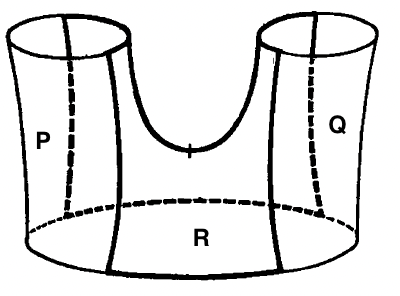
\includegraphics{figures/scan/decoup.png}
    \end{center}
    On prend $\Phi_1 :I\times[a,b]\to P$ et $\Phi_2:J\times[a,b]\to Q$ des homéomorphismes et 
    on pose 
    \[
        \left\lbrace\begin{array}{c c } 
            \Phi(y,t) &y\in K,\\ 
            \Phi_1(y,t) & y\in I,\\ 
            \Phi_2(y,t) & y\in J.
        \end{array}\right.
    \]
    Cette application $V_a\times [a,b]\to T\cup P\cup Q$ (car $K\cup I\cup J= V_a$) est bien 
    définie et est un homéomorphisme. 
    En remarquant que $T\cup P\cup Q=\overline{W_{a,b}-R}$ puis 
    $M_a\cup T\cup Q\cup P=\overline{M_b-R}$, on obtient, en recollant les cylindres de 
    $V_a\times[a,b]$ avec les composantes de $\overline{M_b-R}$ que $M_b-R$ est homéomorphe 
    à $M_a$ et donc $M_b$ est obtenu en recollant les côtés opposés rectangle $R$ à deux 
    segments de $M_a$ distincts.
\end{proof}

Analysons plus en détail ce qu'il se produit lors du passage d'un point critique d'indice $1$. 

Soit $x$ un point critique d'indice $1$ d'une fonction de Morse $f:S\to\R$. 
On a montré que si $a<b$ sont deux valeurs régulières telles que $W_{a,b}$ ne contient pas 
d'autres points critiques de $f$ que $x$, alors $M_b$ est homéomorphe à l'espace obtenu en 
recollant deux côtés opposés d'un rectangle le long de deux segments $I$ et $J$ du bord de $M_a$. 
Il y a différentes manières de procéder à ce recollement qui vont altérer ou pas le nombre de 
composantes de bord de la variété obtenue. 
Il y a trois cas possibles :
\begin{enumerate}[(i)]
    \item Les segments $I$ et $J$ se trouvent sur deux composantes de bord distinctes. 
    Dans ce cas, l'attachement diminue le nombre de composantes de bord.
    \item Les deux segments $I$ et $J$ font partie de la même composante de bord et le rectangle
    est attaché sans "twist". 
    Faire cet attachement augmente de un le nombre de composantes de bord.
    \item Les segments $I$ et $J$ se trouvent dans la même composante de bord et le 
    rectangle est attaché avec un "twist". 
    Cet attachement ne change pas le nombre de composantes de bord. De plus, une fois cet 
    attachement fait, on trouve une partie de $M_b$ qui est homéomorphe à un ruban de Möbius, 
    ce n'est pas possible lorsque $S$ est orientable.
\end{enumerate}